\documentclass[]{article}
\usepackage{float}
\usepackage{graphicx}
\usepackage[svgnames]{xcolor} 
\usepackage{fancyhdr}
\usepackage{fancyvrb}
\usepackage{forest}
\usepackage{tocloft}
\usepackage[hidelinks]{hyperref}
\usepackage{enumitem}
\usepackage[many]{tcolorbox}
\usepackage{listings }
\usepackage[a4paper, total={6in, 8in} , top = 2cm,bottom = 4cm]{geometry}
%\usepackage[a4paper, total={6in, 8in}]{geometry}
\usepackage{afterpage}
\usepackage{amssymb}
\usepackage{pdflscape}
\usepackage{textcomp}
\usepackage{xecolor}
\usepackage{rotating}
\usepackage[Kashida]{xepersian}
\usepackage[T1]{fontenc}
\usepackage{tikz}
\usepackage[utf8]{inputenc}
\usepackage{PTSerif} 
\usepackage{seqsplit}
\usepackage{changepage}


\usepackage{listings}
\usepackage{xcolor}
\usepackage{sectsty}

\setcounter{secnumdepth}{0}
 
\definecolor{codegreen}{rgb}{0,0.6,0}
\definecolor{codegray}{rgb}{0.5,0.5,0.5}
\definecolor{codepurple}{rgb}{0.58,0,0.82}
\definecolor{backcolour}{rgb}{0.95,0.95,0.92}
\definecolor{blanchedalmond}{rgb}{1.0, 0.92, 0.8}
\definecolor{brilliantlavender}{rgb}{0.96, 0.73, 1.0}
 
\NewDocumentCommand{\codeword}{v}{
\texttt{\textcolor{blue}{#1}}
}
\lstset{language=java,keywordstyle={\bfseries \color{blue}}}

\lstdefinestyle{mystyle}{
    backgroundcolor=\color{backcolour},   
    commentstyle=\color{codegreen},
    keywordstyle=\color{magenta},
    numberstyle=\tiny\color{codegray},
    stringstyle=\color{codepurple},
    basicstyle=\ttfamily\normalsize,
    breakatwhitespace=false,         
    breaklines=true,                 
    captionpos=b,                    
    keepspaces=true,                 
    numbers=left,                    
    numbersep=5pt,                  
    showspaces=false,                
    showstringspaces=false,
    showtabs=false,                  
    tabsize=2
}

\lstset{style=mystyle}

 \settextfont[BoldFont={XB Zar bold.ttf}]{XB Zar.ttf}


\setlatintextfont[Scale=1.0,
 BoldFont={LiberationSerif-Bold.ttf}, 
 ItalicFont={LiberationSerif-Italic.ttf}]{LiberationSerif-Regular.ttf}





\newcommand{\inputsample}[1]{
    ~\\
    \textbf{ورودی نمونه}
    ~\\
    \begin{tcolorbox}[breakable,boxrule=0pt]
        \begin{latin}
            \large{
                #1
            }
        \end{latin}
    \end{tcolorbox}
}

\newcommand{\outputsample}[1]{
    ~\\
    \textbf{خروجی نمونه}

    \begin{tcolorbox}[breakable,boxrule=0pt]
        \begin{latin}
            \large{
                #1
            }
        \end{latin}
    \end{tcolorbox}
}

\newtcolorbox{mybox}[2][]{colback=red!5!white,
colframe=red!75!black,fonttitle=\bfseries,
colbacktitle=red!85!black,enhanced,
attach boxed title to top center={yshift=-2mm},
title=#2,#1}

\newenvironment{changemargin}[2]{%
\begin{list}{}{%
\setlength{\topsep}{0pt}%
\setlength{\leftmargin}{#1}%
\setlength{\rightmargin}{#2}%
\setlength{\listparindent}{\parindent}%
\setlength{\itemindent}{\parindent}%
\setlength{\parsep}{\parskip}%
}%
\item[]}{\end{list}}


\definecolor{foldercolor}{RGB}{124,166,198}
\definecolor{sectionColor}{HTML}{ff5e0e}
\definecolor{subsectionColor}{HTML}{008575}

\definecolor{listColor}{HTML}{00d3b9}

\definecolor{umlrelcolor}{HTML}{3c78d8}

\definecolor{subsubsectionColor}{HTML}{3c78d8}

\defpersianfont\authorFont[Scale=0.9]{XB Zar bold.ttf}

\defpersianfont\titr[Scale=1.5]{Lalezar-Regular.ttf}

\defpersianfont\fehrest[Scale=1.2]{Lalezar-Regular.ttf}

\defpersianfont\fehrestTitle[Scale=3.0]{Lalezar-Regular.ttf}

\defpersianfont\fehrestContent[Scale=1.2]{XB Zar bold.ttf}


\sectionfont{\color{sectionColor}}  % sets colour of sections
\subsectionfont{\color{subsectionColor}}  % sets colour of sections
\subsubsectionfont{\color{subsubsectionColor}}


\renewcommand{\labelitemii}{$\circ$}


\renewcommand{\baselinestretch}{1.1}


\renewcommand{\contentsname}{فهرست}

\renewcommand{\cfttoctitlefont}{\fehrestTitle}


\renewcommand\cftsecfont{\color{sectionColor}\fehrestContent\selectfont}
\renewcommand\cftsubsecfont{\color{subsectionColor}\fehrestContent\selectfont}
\renewcommand\cftsubsubsecfont{\color{subsubsectionColor}\fehrestContent\selectfont}
%\renewcommand{\cftsecpagefont}{\color{sectionColor}}

\setlength{\parskip}{1.2pt}

\begin{document}


%%% title pages
\begin{titlepage}
\begin{center}

\textbf{ \Huge{به نام خدا} }
        
\vspace{0.2cm}


\includegraphics[width=0.4\textwidth]{sharif1.png}\\
\vspace{0.2cm}
\textbf{ \Huge{\emph درس برنامه‌سازی پیشرفته} }\\
\vspace{0.25cm}
\textbf{ \Large{ فاز اول پروژه} }
\vspace{0.2cm}
       
 
      \large \textbf{دانشکده مهندسی کامپیوتر}\\\vspace{0.1cm}
    \large   دانشگاه صنعتی شریف\\\vspace{0.2cm}
       \large   ﻧﯿﻢ سال دوم 01-00 \\\vspace{0.10cm}
      \noindent\rule[1ex]{\linewidth}{1pt}
استاد:\\
    \textbf{{دکتر محمدامین فضلی}}



    \vspace{0.20cm}

   مهلت ارسال:\\
    \textbf{{چک پوینت 1: 2 اردیبهشت}}\\
    \textbf{{چک پوینت 2: 11 اردیبهشت}}\\
    \textbf{{فاز اول: 16 اردیبهشت}}\\
    \textbf{{ساعت 23:59:59}}

    \vspace{0.10cm}
مسئول پروژه:\\
    \textbf{\authorFont{امیرمهدی کوششی}}
    
        \vspace{0.10cm}
مسئول فاز اول:\\
    \textbf{\authorFont{آرمان بابایی}}
    
        \vspace{0.10cm}
طراحان فاز اول:\\
    \textbf{\authorFont{علی پاشا منتصری، رضا وحیدی مجد، حسین گلی، امیرمحمد افلاطونیان، امیرمحمد فخیمی، زهرا اذر، مهدی صابر، درین ستوده، پوریا ممتاز، امیررضا ابوطالبی، علی بنافتی‌زاده، ابوالفضل قلندری}}
    
        \vspace{0.05cm}
مسئولین تنظیم مستند:\\
    \textbf{\authorFont{امیرمهدی کوششی، هیربد بهنام، ناصر کاظمی، علی ثالثی}}
    

\end{center}
\end{titlepage}
%%% title pages


%%% header of pages
\newpage
\pagestyle{fancy}
\fancyhf{}
\fancyfoot{}
\cfoot{\thepage}
\lhead{فاز اول}
\rhead{
\includegraphics[width=0.1\textwidth]{sharif.png}\\
دانشکده مهندسی کامپیوتر
}
\chead{پروژه برنامه‌سازی پیشرفته}
%%% header of pages
\renewcommand{\headrulewidth}{2pt}

\KashidaOff



\tableofcontents

\newpage

 \Large \textbf{\\\\
}


\section*{{\titr نکات قابل توجه}}
\addcontentsline{toc}{section}{{\fehrestContent نکات قابل توجه}}
\begin{itemize}
\item
پس از اتمام این فاز، در گیت خود یک تگ با ورژن \lr{"v1.0.0"} بزنید. در روز تحویل حضوری این tag بررسی خواهد شد و کدهای پس از آن نمره‌ای نخواهد گرفت. برای اطلاعات بیش‌تر در مورد شیوه ورژن‌گذاری، می‌توانید به
 \href{https://semver.org/}{\textcolor{blue}{\underline{این لینک}}}
 مراجعه کنید. البته برای این پروژه صرفا رعایت کردن همان ورژن گفته شده کافیست، اما خوب‌ است که با منطق ورژن‌بندی هم آشنا بشوید.

\item
در روز تحویل حضوری مشارکت تمام اعضای تیم در پروژه بررسی خواهد‌ شد و در صورت عدم مشارکت بعضی از اعضا، نمره‌ی ایشان برای آن فاز پروژه "صفر" لحاظ می‌گردد. مشارکت، با توجه به commit های افراد تیم در مخزن گیت‌هاب پروژه بررسی می‌شود.

\item
در هر فاز می‌توانید سه روز تاخیر به ازای کسر نمره داشته‌ باشید که به ازای هر روز آن، ۱۰ درصد از نمرهٔ آن فاز را از دست خواهید‌ داد. در مجموع سه‌فاز پروژه، سه روز تاخیر نیز بخشیده خواهد‌ شد.

\item
به ازای هر ساعتی که پروژه را زودتر تحویل دهید، ۱۵ دقیقه به مهلت تاخیر بدون کسر نمره شما اضافه خواهد‌ شد. این مقدار حداکثر یک روز خواهد‌ بود که در صورت ارسال ۴ روز زودتر از ددلاین به شما تعلق خواهد گرفت. \textbf{بنابراین ددلاین‌های پروژه تحت هیچ شرایطی تمدید نخواهد‌ شد.} توصیه می‌شود با برنامه‌ریزی مناسب به ددلاین‌های درس پایبند باشید.

\item
در صورت کشف تقلب از هریک از تیم‌ها، برای بار اول منفی نمرهٔ آن فاز برای آن تیم ثبت می‌شود و برای بار دوم، نمرهٔ منفی کل پروژه برای تیم لحاظ خواهد‌ شد که معادل مردود شدن در درس است.


\item
شما باید \textbf{حداقل} برای یکی از فرایندهای موجود در پروژه، \lr{Unit Test} بنویسید. همچنین برای \lr{code coverage} بالاتر از ۷۰ درصد، به صورت خطی با درصد \lr{coverage}، نمره‌ٔ امتیازی تعلق خواهد گرفت.

\end{itemize}

\newpage

\section*{{\titr مقدمه}}
\addcontentsline{toc}{section}{{\fehrestContent مقدمه}}

\subsection*{{\titr اهداف پروژه}}

\addcontentsline{toc}{subsection}{{\fehrestContent اهداف قابل توجه}}

\begin{itemize}

\item
هدف این پروژه، طراحی یک بازی مشابه عنوان civilization است. فاز اول به شکل عمده به منطق بازی اختصاص دارد. 

\item
در این فاز از پروژه، طراحی شی‌ءگرای بازی و جداسازی صحیح منطق بخش‌های مختلف از یکدیگر مورد نظر است.

\item
یکی از اهداف پروژه، آشنایی با برخی ابزارها و Pattern های استاندارد برنامه‌نویسی، مثل ابزار مدیریت و تعریف پروژه‌ٔ 
\href{https://en.wikipedia.org/wiki/Apache_Maven}{\textcolor{blue}{\underline{\lr{Apache Maven}}}}، 
است.

\item
آشنایی با سیستم مدیریت نسخه \lr{Git} و کار تیمی بر روی پروژه بر بستر یک مخزن \lr{Github}، یکی از اهداف مهم پروژه است. در این مورد توصیه می‌شود تغییرات خود را در دوره‌های کوتاه مدت \lr{commit} کنید.

\end{itemize}

\subsection*{{\titr کلیات پروژه}}
\addcontentsline{toc}{subsection}{{\fehrestContent کلیات پروژه}}

در این فاز، صرفا منطق پروژه، بدون پیاده‌سازی گرافیک یا معماری شبکهٔ آن، باید پیاده‌سازی شود. نحوهٔ ارتباط با کاربر نیز از طریق واسط کاربری کنسول است. توجه داشته باشید که در فاز سوم پروژه، باید سیستم را طبق یک معماری سرور-کلاینت طراحی کنید. در معماری اکثر بازی‌هایی که به این شکل انجام می‌شوند، منطق بازی در سرور و مستقل از واسط کاربری سمت کلاینت و کاربر است. هر چند برای فاز اول نیاز به این مسئله ندارید ولی خوب‌ است که از الآن طراحی خوبی داشته باشید که قسمت‌های مختلف پروژه نظیر منطق اصلی انجام بازی، وابستگی اساسی به بخش‌هایی نظیر واسط کاربری نداشته باشد. مثلا در فاز‌ آخر پروژه باید امکان چت (\lr{Global Chat}) میان کاربران فراهم 
شود؛ اما برای این فاز با توجه به نبود شبکه، نیازی به پیاده‌سازی آن نیست.

همچنین توجه کنید که در فاز دوم قرار است برای منطق بازی که در این فاز طراحی شده است، رابط کاربری گرافیکی طراحی کنید. در نتیجه جداسازی درست منطق بازی از رابط کاربری آن باعث می‌شود که در فاز ۲ نیاز به بازنویسی کدهای منطق به شدت کاهش یابد. 

در ادامهٔ مستند، موجودیت‌ها، نمای کلی رابط کاربری سیستم، نقش‌ها و دستورات لازم شرح داده‌شده است.

\begin{enumerate}[label={نکته \arabic*:}]
	\item
دقت کنید که دو داک در اختیار شما قرار می گیرد، یک داک توضیحات کاملی از بازی است، و همه چیز راجع به بازی در آن توضیح داده شده است، یک داک دیگر مربوط به فاز اول پروژه شما می باشد که همین داک است، و در این داک، قسمت هایی از بازی که شما باید در فاز اول پیاده سازی کنید آمده است، دقت کنید چیزهایی که در این داک نیامده است، نیاز نیست در این فاز طراحی کنید و تحویل دهید، فقط به آن ها برای طراحی منطق کد خود، توجه داشته باشید.
	
\item
 تمامی اطلاعات، اعم از اطلاعات کاربران و... باید در خارج از برنامه (مثلا روی فایل) ذخیره شوند و پس از \lr{terminate} شدن برنامه و اجرای مجدد آن، بصورت خودکار اطلاعات قبلی خوانده شود و قابل دسترسی باشد. برای این کار می‌توانید از ابزارهای کار با \lr{Json} در جاوا، مثل
  \href{https://www.tutorialspoint.com/gson/gson_quick_guide.htm}{\textcolor{blue}{\lr{Gson}}}
یا
  \href{https://github.com/amogilev/yagson}{\textcolor{blue}{\lr{YaGson}}}
   استفاده‌ کنید.

\item
شما باید پروژه‌ی خود را بر بستر ابزار \lr{Apache Maven} پیاده‌سازی کنید. همچنین برای اضافه کردن کتابخانه‌های مورد نیاز، \lr{dependency} های مربوطه را به فایل \lr{pom.xml} اضافه کنید.




   

\item
در هر جایی از پروژه می‌توانید هرگونه خلاقیتی را به‌کار ببرید. با این حال توجه کنید که خواسته‌های واضح پروژه بایستی انجام شوند و سیستم ورودی گرفتن و خروجی دادن شما باید مطابق جزییات گفته شده در این مستند باشد.


\item در فاز 1 شما باید از طریق کنسول با برنامه خود ارتباط برقرار کنید، به همین دلیل نیاز به یک سری دستورات مشخص می‌باشد که شما از طریق آن دستورات میتوانید بازی را جلو ببرید. به همین منظور یک شیت از دستورات پیشنهادی که می‌توانید از آن‌ها استفاده کنید در این 
 \href{https://docs.google.com/spreadsheets/d/1RQ39m9OvT02mWJlHSsSx2l5XLD5jJ1ifXRnBlijUy34/edit?usp=drivesdk}{\textcolor{blue}{لینک}}
آمده است. (دقت کنید این دستورات پیشنهادی هستند و شما میتوانید دستورات خود را به سلیقه خود پیاده سازی کنید، اما نباید دستورات شما از یک چهارچوب معین خارج شود، در ادامه نیز بیشتر با این موضوع آشنا خواهید شد.)

\item
در مستند بعضی از دستور‌هایی که مشاهده می‌کنید فرمتی به شکل زیر دارند:

\begin{mybox}[colback=yellow]{دستور}
	
	
	\begin{latin}
		
	user login -{}-username <username> -{}-password <password>
		
	\end{latin}
	
\end{mybox}
درواقع ما زمانی از دو دش استفاده می‌کنیم، که بخواهیم یک فیلد را از ورودی بگیریم، در این دستور دو فیلد username و password به این منظور استفاده می‌شود، در نمونه ای دیگر نیز اگر شما بخواهید به عنوان مثال مشخصات یک خانه را دریافت کنید، میتوانید از \lr{-{}-coordinates <coordinates>} استفاده کنید، شما باید در دستورات ساخت خودتان نیز برای گرفتن یک فیلد از دو دش استفاده کنید. (این یک نمونه از همان چهارچوبی است که شما باید در ساخت دستورات خود به آن توجه کنید.)
همچنین در چنین مواردی که شامل پارامتر‌هایی هستند که با
\lr{-{}-}
یعنی دو کاراکتر دش، مشخص شده‌اند، باید بتوانیم از دستور با هر ترتیبی استفاده کنیم. (یعنی دستور زیر

\begin{mybox}[colback=yellow]{دستور}
	
	
	\begin{latin}
		
		user login -{}-password <password> -{}-username <username> 
		
	\end{latin}
	
\end{mybox}

هم دستور معتبری است.

همچنین به عنوان نمره امتیازی، می‌توانید حالت مخفف شده را هم برای آنان پیاده‌سازی کنید. نحوه مخفف سازی به صورت تک حرفی با و با یک نماد -
خواهد بود و نحوه انتخاب حروف برعهده خودتان است. مثلا برای نمونه بالا چنین عبارتی می‌تواند پیشنهاد خوبی باشد:

\begin{mybox}[colback=yellow]{دستور}
	
	
	\begin{latin}
		
		user login -p <password> -u <username> 
		
	\end{latin}
	
\end{mybox}

همچنین توجه کنید که اگر دستور نامعتبری وارد شد که در قسمت مربوطه، برای آن خطای به خصوصی در نظر گرفته نشده بود، پیام زیر را چاپ کنید:

\begin{mybox}[colback=yellow]{پیغام به کاربر}
	
	
	\begin{latin}
		
	invalid command
		
	\end{latin}
	
\end{mybox}


\end{enumerate}




\newpage


\section*{{\titr معرفی بازی}}
\addcontentsline{toc}{section}{{\fehrestContent معرفی بازی}}

در مستند ضمیمه، به معرفی بازی و قواعد آن مستقل از خواسته‌های پروژه پرداخته شده است. توصیه می‌شود قبل از مطالعه این مستند که در مورد نکات پیاده‌سازی خود پروژه است، به مطالعه داک مربوط به بازی بپردازید.





\section*{{\titr توضیح بخش‌های مختلف پروژه}}
\addcontentsline{toc}{section}{{\fehrestContent توضیح بخش‌های مختلف پروژه}}



\subsection*{{\titr کاربر، منوها و موارد عمومی}}
\addcontentsline{toc}{subsection}{{\fehrestContent کاربر، منوها و موارد عمومی
}}

در این بازی مانند تمام بازی‌های دیگر یک عده کاربر وجود دارند که بازی می‌کنند. 
هر کاربر باید فیلد‌های زیر را داشته باشد:
\begin{itemize}[label=$\blacksquare$]
	\begin{latin}
		\item username
		\item password
		\item nickname
		\item score
	\end{latin}
\end{itemize}
 \forestset{
	declare dimen register=folder indent,
	folder indent=.45em,
	folder/.style={
		parent anchor=-children last,
		anchor=parent first,
		calign=child,
		calign primary child=1,
		for children={
			child anchor=parent,
			anchor=parent first,
			edge={rotate/.option=!parent.grow},
			edge path'/.expanded={
				([xshift=\forestregister{folder indent}]!u.parent anchor) |- (.child anchor)
			},
		},
		after packing node={
			if n children=0{}{
				tempdiml=l_sep()-l("!1"),
				tempdims={-abs(max_s("","")-min_s("",""))-s_sep()},
				for children={
					l+=tempdiml,
					s+=tempdims()*(reversed()-0.5)*2,
				},
			},
		},
	}
}
در ابتدای بازی هر فرد باید ثبت نام کند و سپس در دفعات بعدی فقط وارد شود و 
بازی کند.
\\
پس از ورود به بازی، وارد منوی ورود و ثبت‌نام (\lr{Login Menu}) می‌شویم و پس از 
ساخت اکانت و وارد شدن کاربر به منوی اصلی (\lr{Main Menu}) می‌رویم که راه 
ارتباطی میان تمام اجزای مختلف بازی است. توجه کنید اگر کاربر بدون لاگین کردن قصد رفتن به منوی دیگری را داشته باشد، باید با خطای زیر رو به رو شود:
\begin{mybox}[colback=yellow]{پیغام به کاربر}
	\begin{latin}	
		please login first
	\end{latin}
\end{mybox}
\newpage
 در کل ساختار منوهای ما به شکل زیر است:

\begin{latin}
	
	\begin{forest}
		for tree={grow'=0,folder,draw}
		[Login
		[Main
		[Play Game]
		[Profile]
		]
		]
	\end{forest}
\end{latin}

دستورات هر منو فقط داخل آن‌ها معتبر است و اگر در منوی مربوطه صدا زده نشوند، 
باید خطای مناسب چاپ شود.

\subsubsection*{{\titr دستورات مرتبط با منو}}
\addcontentsline{toc}{subsubsection}{{\fehrestContent دستورات مرتبط با 
منو}}
\vspace{.5cm}
\textbf{ورود به یک منو:}
\begin{mybox}[colback=yellow]{دستور}
	\begin{latin}	
		menu enter <menu name>
	\end{latin}
\end{mybox}


در صورتی که کاربر داخل یک منوی دیگر باشد باید خطای زیر چاپ شود:
\\
\begin{mybox}[colback=yellow]{پیغام به کاربر}
	\begin{latin}	
		menu navigation is not possible
	\end{latin}
\end{mybox}

\vspace{.5cm}
\textbf{خروج از یک منو:}
\begin{mybox}[colback=yellow]{دستور}
	\begin{latin}	
		menu exit
	\end{latin}
\end{mybox}
در صورتی داخل یک منو باشیم، این دستور ما را به منوی بالاتر می‌برد و اگر در 
منوی اصلی باشیم وارد منوی ورود و ثبت‌نام خواهیم شد. در صورتی که در منوی 
ورود 
و ثبت‌نام بودیم، بازی خاتمه خواهد یافت.

\vspace{.5cm}
\newpage
\textbf{منوی فعلی:}
\begin{mybox}[colback=yellow]{دستور}
	\begin{latin}	
		menu show-current 
	\end{latin}
\end{mybox}
این دستور نام منوی فعلی را نشان می‌دهد و اگر در منوی اصلی باشیم 
\lr{Main Menu} و اگر در منوی ورود و ثبت‌نام باشیم \lr{Login Menu} چاپ می‌شود.

\vspace{.5cm}
\textbf{ساخت کاربر جدید:}
\begin{mybox}[colback=yellow]{دستور}
	\begin{latin}	
		user create -{}-username <username> -{}-nickname <nickname> 
		-{}-password 
		<password>
	\end{latin}
\end{mybox}
پیغام موفقیت:
\begin{mybox}[colback=yellow]{پیغام به کاربر}
	\begin{latin}	
		user created successfully!
	\end{latin}
\end{mybox}
خطا‌های زیر در صورت وجود به همین ترتیب بررسی شوند:
\\
نام کاربری تکراری:
\begin{mybox}[colback=yellow]{پیغام به کاربر}
	\begin{latin}	
		user with username <username> already exists
	\end{latin}
\end{mybox}
نام مستعار تکراری:
\begin{mybox}[colback=yellow]{پیغام به کاربر}
	\begin{latin}	
		user with nickname <nickname> already exists
	\end{latin}
\end{mybox}

\vspace{.5cm}
\textbf{ورود کاربر:}
\begin{mybox}[colback=yellow]{دستور}
	\begin{latin}	
		user login -{}-username <username> -{}-password <password>
	\end{latin}
\end{mybox}
پیغام موفقیت:
\begin{mybox}[colback=yellow]{پیغام به کاربر}
	\begin{latin}	
		user logged in successfully!
	\end{latin}
\end{mybox}
خطا‌های زیر در صورت وجود به همین ترتیب بررسی شوند:
\\
عدم وجود کاربر با این نام کاربری:
\begin{mybox}[colback=yellow]{پیغام به کاربر}
	\begin{latin}	
		Username and password didn’t match!
	\end{latin}
\end{mybox}
رمز اشتباه:
\begin{mybox}[colback=yellow]{پیغام به کاربر}
	\begin{latin}	
		Username and password didn’t match!
	\end{latin}
\end{mybox}
توجه کنید که از دیدگاه امنیت، یک تلاش ناموفق برای ورود هیچ‌گاه نباید دارای 
اطلاعاتی باشد که فرایند ورود را برای بار دوم راحت‌تر کند. مثلا اگر فردی 
صرفا 
قصد دزدیدن یکسری اکانت بدون توجه به صاحب آن‌ها را داشته باشد و در نتیجه 
یکسری نام‌کاربری تصادفی را امتحان کند، در صورتی که نام‌کاربری و پسورد مطابقت 
نداشت، نباید از پیام ما متوجه بشود که نام‌کاربری که وارد کرده، واقعا در 
سیستم وجود دارد. در نتیجه در هر دو حالت بالا پیغام خطای یکسانی چاپ می‌شود.

\vspace{.5cm}
\textbf{خروج کاربر:}
\begin{mybox}[colback=yellow]{دستور}
	\begin{latin}	
		user logout
	\end{latin}
\end{mybox}
این دستور تنها در منوی اصلی معتبر است و در صورت موفقیت، وارد منوی ورودی و 
ثبت‌نام می‌شود.
\\
پیغام موفقیت:
\begin{mybox}[colback=yellow]{پیغام به کاربر}
	\begin{latin}	
		user logged out successfully!
	\end{latin}
\end{mybox}

\vspace{.5cm}
\textbf{بازی:}
\\
همانطور که گفته شد، این بازی یک بازی چند نفره است، لذا شما باید یوزرنیم افرادی که میخواهید با آن‌ها بازی کنید را داشته باشید تا به صورت زیر وارد بازی شوید.\\

\begin{mybox}[colback=yellow]{دستور}
	\begin{latin}	
		play game -{}-player1 <username> -{}-player2 <username>
	\end{latin}
\end{mybox}
\newpage
\noindent \textbf{دقت کنید} اگر تعداد افرادی که قرار بود با آن‌ها بازی کنید، بیشتر بود، نیاز است که به همین ترتیب در دستور شروع بازی، ابتدا \lr{-{}-player} و سپس شماره آن بازیکن و سپس بعد از آن یوزرنیم آن را وارد کنید.\\
 در صورتی که یک یا چند یوزرنیم وجود نداشت پیغام خطای مناسب به کاربر نشان داده شود. و همینطور در صورت ورود به بازی نیز پیغام مناسب چاپ شود.\\
\vspace{.5cm}
\textbf{پروفایل:}
\\
پس از ورود به منوی profile دستورات زیر معتبر هستند:
\\
\\
\vspace{.5cm}
\textbf{تغییر نام مستعار:}
\begin{mybox}[colback=yellow]{دستور}
	\begin{latin}	
		profile change -{}-nickname <nickname>
	\end{latin}
\end{mybox}
پیغام موفقیت:
\begin{mybox}[colback=yellow]{پیغام به کاربر}
	\begin{latin}	
		nickname changed successfully!
	\end{latin}
\end{mybox}
در صورتی که کاربری با این نام مستعار وجود داشت خطای زیر چاپ شود:
\begin{mybox}[colback=yellow]{پیغام به کاربر}
	\begin{latin}	
		user with nickname <nickname> already exists
	\end{latin}
\end{mybox}

\vspace{.5cm}
\textbf{تغییر رمز عبور:}
\begin{mybox}[colback=yellow]{دستور}
	\begin{latin}	
		profile change -{}-password -{}-current <current password> -{}-new <new 
		password>
	\end{latin}
\end{mybox}
پیغام موفقیت:
\begin{mybox}[colback=yellow]{پیغام به کاربر}
	\begin{latin}	
		password changed successfully!
	\end{latin}
\end{mybox}
خطا‌های زیر در صورت وجود به همین ترتیب بررسی شوند:
\\
نادرست بودن رمز فعلی:
\begin{mybox}[colback=yellow]{پیغام به کاربر}
	\begin{latin}	
		current password is invalid
	\end{latin}
\end{mybox}
یکی بودن رمز قدیم و جدید:
\begin{mybox}[colback=yellow]{پیغام به کاربر}
	\begin{latin}	
		please enter a new password
	\end{latin}
\end{mybox}

\newpage 
\subsection*{{\titr نقشه بازی}}
\addcontentsline{toc}{subsection}{{\fehrestContent نقشه بازی}}
پیشنهاد ما این است که نقشه‌ی کوچکی در ترمینال خود نمایش دهید، و با هر دستور جدید این نقشه را بروز کنید و بعد از ابتدا چاپ کنید.

نقشه‌ی شما می‌تواند عنصرهای مختلف درون نقشه را به صورت رنگ، حروف اختصاری، و یا کلمات کامل نشان دهد. همچنین می‌توانید برخی از اطلاعات را به زمان انتخاب شدن یک کاشی واگذار کنید. پیشنهاد می‌شود که مختصات هر خانه را چاپ کنید تا انتخاب یک خانه‌ی خاص در دستورات ممکن باشد.
مثلا یک نقشه‌ی ممکن می‌تواند مانند شکل زیر باشد:
\begin{figure}[H]
    \centerline{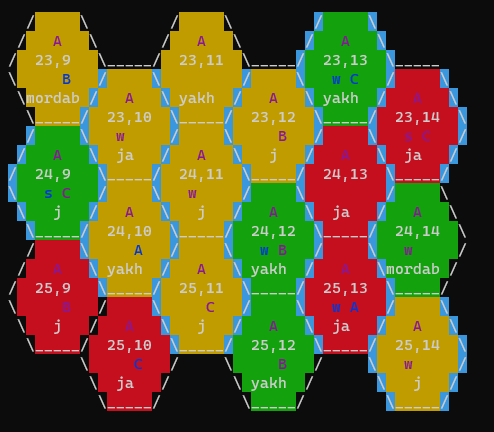
\includegraphics[scale=0.8]{Resources/map.png}}
\end{figure}
به طور مثال کاشی بالا سمت چپ نقشه، در مختصات 23,9 قرار دارد. این کاشی در محدوده‌ی مرزهای تمدن \lr{A} (با رنگ بنفش) است، در زمین صحرایی (با توجه به رنگ زرد پس‌زمینه‌ی آن)  واقع شده و ویژگی مرداب را دارا است. در این خانه یک یگان نظامی از نوع \lr{Ballista} قرار دارد که مربوط به تمدنی‌ست که رنگ آبی را دارد (حرف \lr{B})، اما یگان غیرنظامی‌ای در آن وجود ندارد. در ضلع پایین سمت راست این کاشی، یک رودخانه واقع شده است که با رنگ پس‌زمینه‌ی آبی مشخص شده است.
از طرف دیگر، کاشی پایینی آن در مختصات 24,9 در زمین علفزار (با توجه به رنگ سبز پس‌زمینه‌ی آن) قرار دارد. در این کاشی که از ویژگی جنگل (با توجه به حرف \lr{j}) برخوردار است، یک یگان غیرنظامی مهاجر متعلق به تمدن آبی (با توحه به حرف \lr{s}) و با توجه به حرف \lr{C} یک واحد نظامی \lr{Catapult} متعلق به تمدن بنفش (همان \lr{A}) قرار دارد.
شما باید نقشه‌ای مثل شکل بالا ایجاد کنید. البته شما در انتخاب این که چطور می‌خواهید اطلاعات درون نقشه را نشان دهید، مختارید. مثلا می‌توانید رودخانه‌ها را به جای رنگ پس‌زمینه، با مرزهای «-» برای کاشی نشان دهید. یا به جای استفاده از رنگ پس‌زمینه برای نشان دادن نوع زمین، این اطلاعات را به طور مستقیم روی نقشه بنویسید. آن‌چه که در نهایت اهمیت دارد این است که \textbf{وضعیت رودخانه‌ها، مالکیت زمین‌ها، یگان‌های موجود در کاشی و مالکیت آن‌ها، مختصات کاشی، نوع زمین کاشی، ویژگی زمین کاشی، منبع موجود در کاشی و پیشرفت‌های موجود در کاشی  در نقشه مشخص باشد.}

\subsection*{\titr کد تقلب}
\addcontentsline{toc}{subsection}{{\fehrestContent کد تقلب}}
احتمالا در بازی های زیادی دیدید (شنیدید) که یک سری کدهای تقلب وجود دارد که بازی را از حالت عادی خارج می‌کند، نمونه ای از این کد ها مثلا در بازی GTA وجود دارد، می‌تواند باعث شود تمامی اسلحه‌ها برای بازکن در دسترس باشد، یا در مثال دیگر می‌تواند باعث شوند بازیکن هیچگاه جان خودش را از دست ندهد. در پروژه شما نیز این قابلیت باید پیاده سازی شود. در این حالت پروژه شما باید بتواند کارهایی که در حالت عادی نمی‌توانید انجام دهد را پیاده سازی کند، نمونه ای از این کار‌ها را می‌توان افزایش پول به مقدار دلخواه، گذشتن چند نوبت پشت سر هم، پیروزی در یک نبرد، به دست اوردن غذا و تکنولوژی و ... باشد. در اینجا نمونه‌ای از دستورات پیشنهادی را برای شما آورده‌ایم. شما نیز می‌توانید خودتان دستورات دیگری برای این حالت توسعه دهید و در زمینه های دیگر استفاده کنید. (دقت کنید برای تمام فعالیت‌های بازی اعم از برد یک دست بازی، حرکت یگان‌ها، ساختمان‌ها، یونیت‌ها، شهرها و... کد تقلب داشته باشید.)\\
جلو رفتن نوبت‌های بازی:
\begin{mybox}[colback=yellow]{دستور}
	\begin{latin}	
		increase --turn <amount>
	\end{latin}
\end{mybox}
زیاد شدن پول:
\begin{mybox}[colback=yellow]{دستور}
	\begin{latin}	
		increase --gold <amount>
	\end{latin}
\end{mybox}

\subsection*{\titr مواردی که باید در فاز 1 پیاده سازی شوند}
\addcontentsline{toc}{subsection}{{\fehrestContent پیاده سازی فاز 1}}
برای راحتی کار شما، در فاز اول، یک سری موارد کلی ای از بازی پیاده سازی می‌شوند که در واقع همان منطق اصلی بازی هستند، و سایر موارد به ترتیب در فازهای بعدی پروژه تکمیل می‌شوند.\\
علاوه بر موارد مخصوص به فاز 1 که در همین داک دیدید (منوها، نقشه بازی، کدهای تقلب) شما باید مواردی از داک بازی نیز که مربوط به فاز 1 هست را نیز پیاده سازی کنید.\\
در واقع بازی پیاده سازی شده در فاز 1 به شکلی به طور کلی اینگونه می‌باشد:\\
کاربران می‌توانند برای خودشان یک سری یوزر در بازی بسازند، اطلاعاتشان را عوض کنند، با سایر کاربران بازی کنند. در محیط بازی نیز در فاز 1 شما باید زمین‌ها، ویژگی‌های آن‌ها، یگان‌ها، منابع، حرکت یگان‌ها بر روی زمین، منابع، تکنولوژی را داشته باشید. در فاز 1 برد و باخت یک تمدن  حمله کردن تمدن‌ها و یگان‌های نظامی به یکدیگر چک نمی‌شوند و شما باید آن‌ها را در فازهای بعدی پروژه تکمیل کنید.\\
به طور کلی‌تر، موارد زیر را نیاز نیست در فاز 1 پیاده سازی کنید:
\begin{itemize}
    \item برخی از اعمال تمدن‌ها (معامله کردن با یک تمدن دیگر، جنگ)
    \item برد و باخت در بازی
    \item خرابه‌ها(ruins)
    \item ساختمان‌ها
\end{itemize}

\section*{\titr چک پوینت}
\addcontentsline{toc}{section}{{\fehrestContent چک پوینت}}

یکی از مواردی که در این پروژه باید به آن دقت کنید، چک پوینت‌ها هستند. در واقع چک پوینت‌ها همان ددلاین‌های تقسیم شده در طول هر فاز می‌باشند. از شما خواسته می‌شود با توجه به زمان پایان هر چک پوینت، مواردی از فاز اول پروژه که در آن چک پوینت باید زده شوند را، با تگ "\lr{CP\#.0.0}" در مخزن گیت‌هاب خود قرار دهید.\\
در این فاز، شما 2 چک پوینت و یک ددلاین پایانی فاز 1 را دارید. همچنین هر چک پوینت نیز میزان نمره‌ای از کل نمره پروژه دارد.\\
مواردی که باید تا پایان زمان هر چک پوینت زده شوند در زیر آمده است.

\newpage
\subsection*{\titr چک پوینت 1}
\addcontentsline{toc}{subsection}{{\fehrestContent چک پوینت 1}}
\begin{itemize}
    \item حجم موارد خواسته شده در این چک پوینت نسبت به کل مطالب این فاز: 40\%
    \\
    \\
کامل کردن منو ها (تمپلیت) و قابلیت ساخت اکانت وجود دیتابیس \lr{User}ها  و پیاده کردن Map بازی و معماری(لزومی به پیاده سازی کامل نیست صرفا تقریبا مشخص باشد چه تابعایی و چه چیزهایی لازم است) و کلاس های لازم برای Object های اولیه مثل Block - City - Unit پیاده سازی Movement and Exploration ( توانایی حرکت دادن نیرو ها در MAP و war of fog ) هر نوع نیرو یک کلاس پدر Unit دارد و توانایی دستور دادن به این کلاس کلی مد نظر است (پیاده سازی نیروهای جنگی در ادامه)
\end{itemize}

\subsection*{\titr چک پوینت 2}
\addcontentsline{toc}{subsection}{{\fehrestContent چک پوینت 2}}
  \begin{itemize}  
    \item حجم موارد خواسته شده در این چک پوینت نسبت به کل مطالب این فاز: 30\%
    \\
    \\
    قابلیت احداث شهر و منطق مربوط به شهرها
\end{itemize}
\subsection*{\titr فاز 1}
\addcontentsline{toc}{subsection}{{\fehrestContent فاز 1}}
 \begin{itemize}   
    \item حجم موارد خواسته شده در این چک پوینت نسبت به کل مطالب این فاز: 30\%
    \\
    \\
    موارد باقی مانده از پیاده سازی فاز اول پروژه
\end{itemize}




\end{document}







